\documentclass[11pt]{article}
\usepackage{geometry} % Pour passer au format A4
\geometry{hmargin=1cm, vmargin=1cm} % 

% Page et encodage
\usepackage[T1]{fontenc} % Use 8-bit encoding that has 256 glyphs
\usepackage[english,french]{babel} % Français et anglais
\usepackage[utf8]{inputenc} 

\usepackage{lmodern}
\setlength\parindent{0pt}

% Graphiques
\usepackage{graphicx,float,grffile}

% Maths et divers
\usepackage{amsmath,amsfonts,amssymb,amsthm,verbatim}
\usepackage{multicol,enumitem,url,eurosym,gensymb,multido}

% Sections
\usepackage{sectsty} % Allows customizing section commands
\allsectionsfont{\centering \normalfont\scshape}

% Tête et pied de page

\usepackage{fancyhdr} 
\pagestyle{fancyplain} 

\fancyhead{} % No page header
\fancyfoot{}

\renewcommand{\headrulewidth}{0pt} % Remove header underlines
\renewcommand{\footrulewidth}{0pt} % Remove footer underlines

\newcommand{\horrule}[1]{\rule{\linewidth}{#1}} % Create horizontal rule command with 1 argument of height

\newcommand{\Pointilles}[1][3]{%
  \multido{}{#1}{\makebox[\linewidth]{\dotfill}\\[\parskip]
}}

\begin{document}

\subsection*{Ex1}

\textit{Mesurer les côtés, mesurer la hauteur. Calculer l'aire.}

\begin{figure}[H]
  \centering
  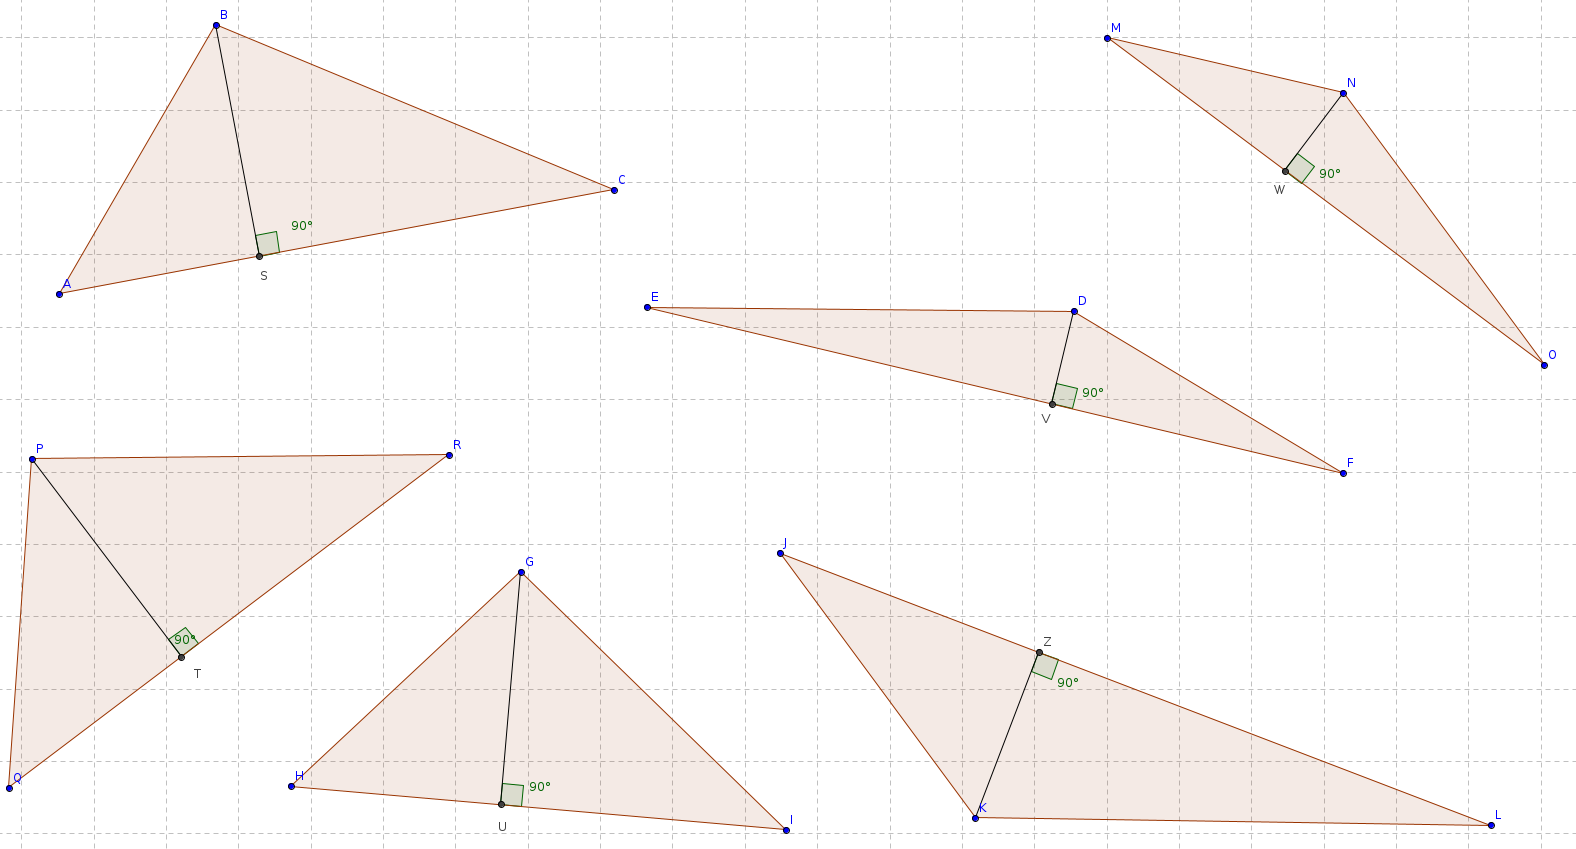
\includegraphics[width=\linewidth]{5x2-triangles/sources/hauteur-1.png}
\end{figure}

\subsection*{Ex2}

\textit{Mesurer les côtés, Tracer une hauteur, mesurer la hauteur. Calculer l'aire.}

\begin{figure}[H]
  \centering
  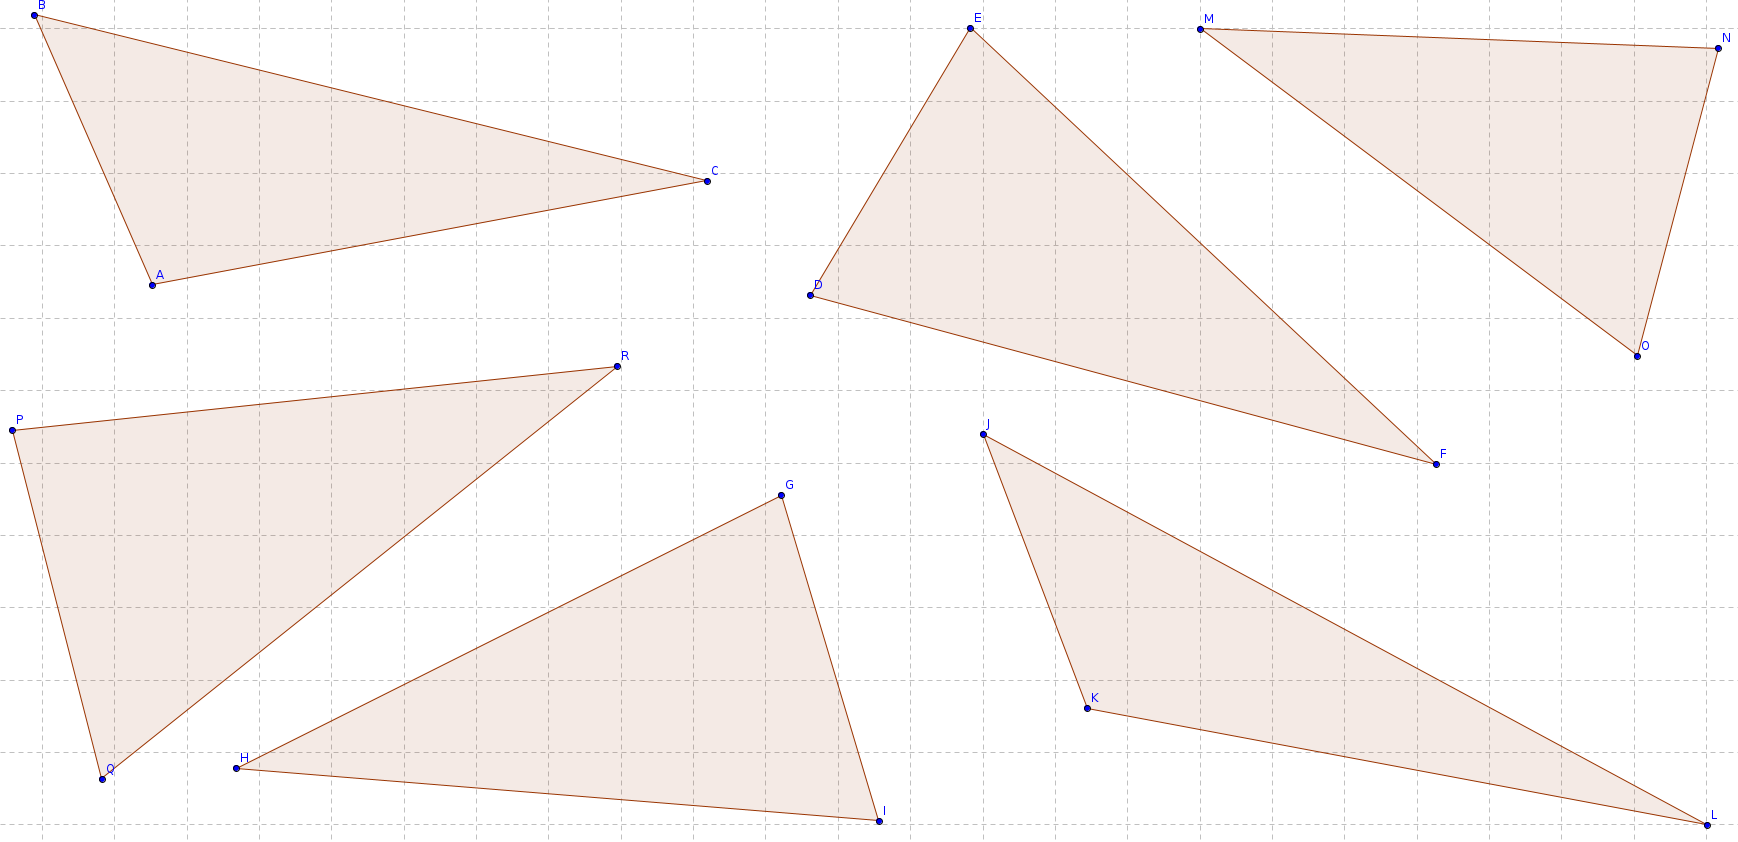
\includegraphics[width=\linewidth]{5x2-triangles/sources/hauteur-2.png}
\end{figure}

\newpage
\subsection*{Ex3}

\textit{Mesurer les côtés, Tracer une hauteur, mesurer la hauteur. Calculer l'aire.}

\begin{figure}[H]
  \centering
  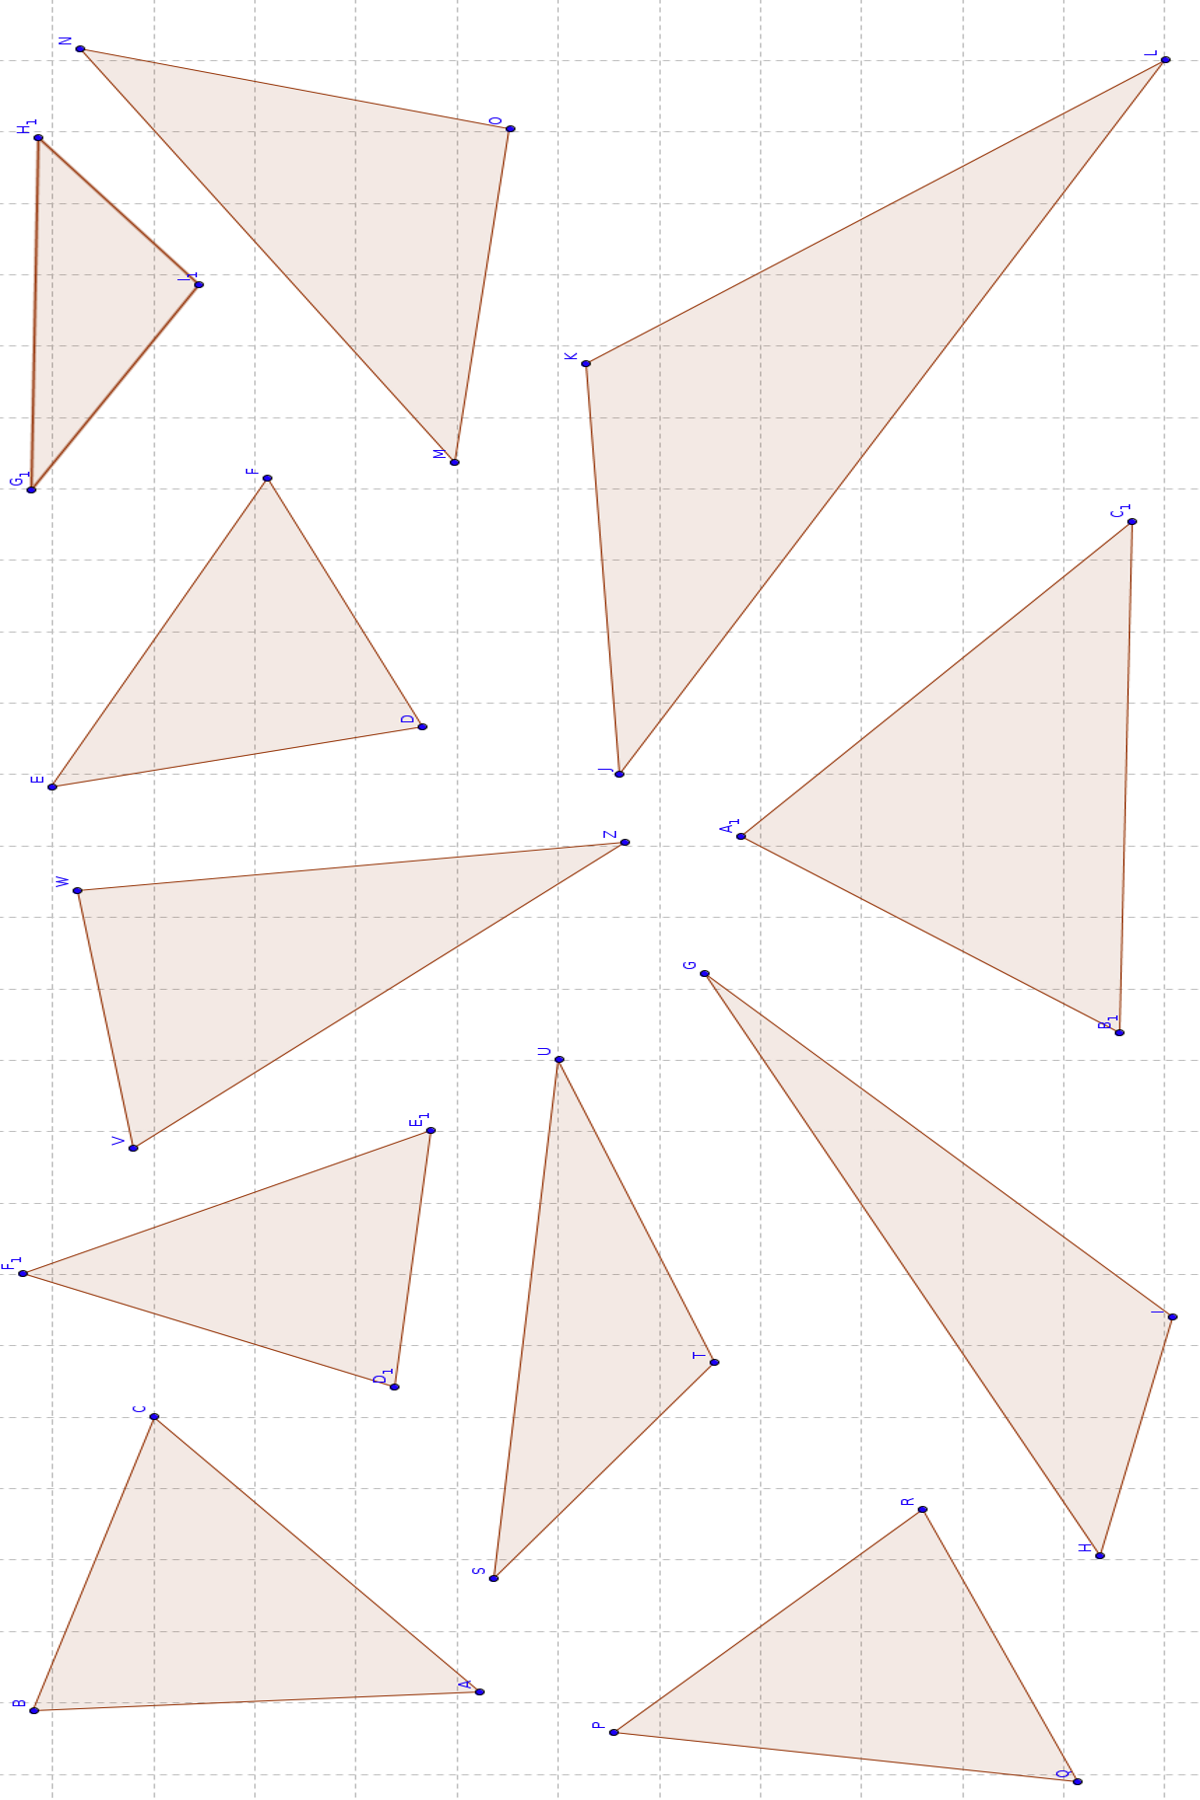
\includegraphics[width=0.8\linewidth]{5x2-triangles/sources/hauteur-3.png}
\end{figure}


\end{document}
